\documentclass[12pt]{article}
\usepackage{amsmath, amssymb, amsthm, epsfig}
\usepackage{listings}
\usepackage{tikz}
\usetikzlibrary{math,decorations.pathreplacing, shapes.geometric}
\usepackage{quiver}
\usepackage{fontspec}
\setmonofont{DejaVu Sans Mono}
\theoremstyle{definition}
\usepackage{enumitem}
\newenvironment{Proof}{\noindent {\sc Proof.}}{$\Box$ \vspace{2 ex}}
\newenvironment{Solution}{\noindent {\sc Solution.}}{$\Box$ \vspace{2 ex}}


\usepackage{color}
\definecolor{keywordcolor}{rgb}{0.7, 0.1, 0.1}   % red
\definecolor{tacticcolor}{rgb}{0.0, 0.1, 0.6}    % blue
\definecolor{commentcolor}{rgb}{0.4, 0.4, 0.4}   % grey
\definecolor{symbolcolor}{rgb}{0.0, 0.1, 0.6}    % blue
\definecolor{sortcolor}{rgb}{0.1, 0.5, 0.1}      % green
\definecolor{attributecolor}{rgb}{0.7, 0.1, 0.1} % red

\def\lstlanguagefiles{../lstlean.tex}

\oddsidemargin-1mm
\evensidemargin-0mm
\textwidth6.5in
\topmargin-15mm
\textheight8.75in
\footskip27pt

\usepackage[table]{xcolor}
\definecolor{truecolor}{RGB}{198,239,206} % Light green
\definecolor{falsecolor}{RGB}{255,199,206} % Light red
\newcommand{\true}{\cellcolor{truecolor}T}
\newcommand{\false}{\cellcolor{falsecolor}F}
\begin{document}

\noindent \textit{\textbf{Math 300, Winter 2026}} \hspace{1.3cm} \textit{\textbf{HOMEWORK 1}} \hspace{1.3cm} 
\textit{\textbf{Grant Yang}
} 

\vspace{1cm}

\begin{Solution}
{\bf (\S1.1, Problem 4)}\\
\textbf{Axiom}: `groan' is true. \\
\textbf{Logic}: Given a true statement, replacing a letter at any place also yields a true statement.
\begin{enumerate}[label=\alph*.]
\item Proof of `cloth': groan,croan,cloan,clotn,cloth $\square$
\item{
    The difference between true and false statements in this system is just their lengths: all 5-letter statements should be true, while statements of any other length should be false. We can produce a proof of any 5-letter statement by starting at 'groan` and repeatedly changing the first letter that does not match, and this process is guaranteed to terminate as we need at most 5 steps. However, since changing letters does not change the statement's length, and since this is the only possible step that we can take, we cannot hope to prove any statement that is not 5 letters long (it is an invariant). With this, we refute the claim that 'xylem` is false by providing a proof for 'xylem`.
}
\end{enumerate}
\end{Solution} 

% \vspace{1cm}

\begin{Solution}
{\bf (\S1.3, Problem 8)}\\
\begin{enumerate}[label=\alph*.]
\item ``Claudia will run in the marathon if she has trained properly or is
injury-free at race time.'' \begin{equation*} \text{(injury free)} \lor \text{(trained properly)} \implies  \text{(runs in marathon)}.\end{equation*}

\item ``Claudia will run in the marathon only if she is injury-free at race
time.'' \begin{equation*} \text{(runs in marathon)} \implies \text{(injury free)}.\end{equation*}
\item ``Claudia will run in the marathon if and only if she has trained properly
and is injury-free at race time.'' \begin{equation*} \text{(injury free)} \wedge \text{(trained properly)} \iff  \text{(runs in marathon)}.\end{equation*}
\end{enumerate}
\end{Solution} 

\vspace{1cm}

\begin{Solution}
{\bf (\S1.3, Problem 10)}\\
\begin{enumerate}[label=\alph*.]
    \item Invalid (unbalanced parens): $(P \implies \lnot Q) \implies ((\lnot(\lnot P)) \iff Q)$ can be made valid as $$(P \implies \lnot Q) \implies (((\lnot(\lnot P)) \iff Q).$$
    \item Invalid (unbalanced parens): $(P \implies Q) \implies R) \implies S) \implies T$ can be made valid as $$(((P \implies Q) \implies R) \implies S) \implies T.$$
    \item Valid statement form: $$(P \implies (\lnot Q \implies R)) \implies Q.$$ (ok, if you're pedantic you can argue that $\lnot Q \implies R$ is ambiguous as it can be parsed as either $\lnot (Q \implies R)$ or $(\lnot Q) \implies R$, but everyone knows it's the latter since $\lnot$ has higher precedence than $\implies$, come on).
    \item Valid statement form: $$((P \implies Q \implies R) \land Q) \lor (\lnot (P \lor Q)).$$ (ok, again if you're pedantic you can argue you don't know if $P \implies Q \implies R$ should be parsed as $(P \implies Q) \implies R$ or as $P \implies (Q \implies R)$, but again everyone knows it's the latter since $\implies$ is right-associative, come on guys).
    \item Valid statement form: $$(\lnot P \lor Q) \iff (((P \land Q) \lor (P \lor R)) \implies (S \lor \lnot P)).$$ Same note about the ambiguity in parsing $\lnot P \lor Q$ as either $\lnot (P \lor Q)$ or $(\lnot P) \lor Q$: it should be the latter as $\lnot$ has higher precedence than $\lor$.
\end{enumerate}
\end{Solution} 

\vspace{1cm}

\begin{Solution}
{\bf (\S1.3, Problem 16)}\\
Given a statement form $S$ with $n \ge 3$ variables $P_1,P_2,\dots,P_n$, then in the truth table for $S$, there are exactly $\boxed{2^{n-1}}$ rows in which $P_1$ is false, and there are exactly $\boxed{2^{n-2}}$ rows in which $P_1$ is false while $P_2$ is true. Each row of the truth table corresponds to one possible distinct choice for the values $\vec P_n$, and since we have $2$ choices (either true or false) for each of the $n$ free variables, we have $2^n$ rows in the truth table for $S$. Fixing $P_1$ to be false leaves $n-1$ free variables and thus $2^{n-1}$ rows, and further fixing $P_2$ to be true leaves $n-2$ free variables and $2^{n-2}$ rows. We know that we started with $n\ge 3$ free variables, so it is valid to remove two of them like this.
\end{Solution} 

\vspace{1cm}

\begin{Solution}
{\bf (\S1.3, Problem 18)}\\
\begin{enumerate}[label=\alph*.]
    \item Yes, $P \implies \lnot P \implies Q$ is a tautology: \\
    \begin{tabular}{|c|c||c|c|c|c|}
    \hline
        $P$ & $Q$ & $\lnot P$ & $\lnot P \implies Q$ & $P \implies \lnot P \implies Q$  \\ \hline
        \false & \false & \true & \false & \true \\ \hline
        \false & \true & \true & \true & \true \\ \hline
        \true & \true & \false & \true & \true \\ \hline
        \true & \false & \false & \true & \true \\ \hline
    \end{tabular}

    \item Yes, $P \land Q \implies P \lor R$ is a tautology: \\
    \begin{tabular}{|c|c|c||c|c|c|c|}
    \hline
        $P$ & $Q$ & $R$ & $P \land Q$ & $P \lor R$ & $P \land Q \implies P \lor R$  \\ \hline
        \false & \false & \false & \false & \false & \true \\ \hline
        \false & \false & \true & \false & \true & \true\\ \hline
        \false & \true & \true & \false & \true & \true \\ \hline
        \false & \true & \false & \false & \true & \true\\ \hline
        \true & \true & \false & \true & \true & \true \\ \hline
        \true & \true & \true & \true & \true & \true\\ \hline
        \true & \false & \true & \false & \true & \true\\ \hline
        \true & \false & \false & \false & \false & \true \\ \hline
    \end{tabular}

    \item No, $((P\implies Q)\iff Q) \implies P$ is not a tautology:

    \begin{tabular}{|c|c||c|c|c|}
        \hline
        $P$ & $Q$ & $P \implies Q$ & $(P \implies Q)\iff Q$ & $((P \implies Q) \iff Q) \implies P$ \\ \hline
        \false&\false&\true&\false&\true\\ \hline
        \false&\true&\true&\true&\false(!) \\ \hline
        \true&\true&\true&\true&\true\\ \hline
        \true&\false&\false&\true&\true\\ \hline
    \end{tabular}

    \item Yes, $P \implies Q \implies Q \implies P$ is a tautology: \\
    \begin{tabular}{|c|c||c|c|c|}
        \hline
        $P$ & $Q$ & $Q \implies P$ & $Q \implies Q \implies P$ & $P \implies Q \implies Q \implies P$ \\ \hline
        \false&\false&\true&\true&\true\\ \hline
        \false&\true&\false&\false&\true\\ \hline
        \true&\true&\true&\true&\true\\ \hline
        \true&\false&\true&\true&\true\\ \hline
    \end{tabular}
\end{enumerate}

\end{Solution} 

\vspace{1cm}

\begin{Solution}
{\bf (\S1.4, Problem 4)}\\
If $n_1$ and $n_2$ are odd, then $n_1 + n_2$ is even. By the definition of odd number, there exist two natural numbers $k_1$ and $k_2$ such that $n_1 = 2 k_1 + 1$ and $n_2 = 2 k_2 + 1$. Then, $n_1 + n_2 = 2 k_1 + 1 + 2 k_2 + 1= 2(k_1+k_2+1)$. Thus, $n_1 + n_2$ is even by the definition of an even number, as $k_1 + k_2 + 1$ is a natural number since the naturals are closed under addition.

If $n_1$ and $n_2$ are even, then there exist $k_1,k_2 \in \mathbb{N}$ such that $n_1 = 2 k_1$ and $n_2 = 2 k_2$. Then $n_1 + n_2 = 2 k_1 + 2 k_2 = 2(k_1 + k_2)$, implying that $n_1+n_2$ is even as $k_1 + k_2 \in \mathbb{N}$.

The sum of an odd number and an even number is odd. WLOG, let $n_1$ be odd and $n_2$ be even. Thus, there exist $k_1, k_2 \in \mathbb{N}$ such that $n_1 = 2 k_1 + 1$ and $n_2 = 2 k_2$. Then, $n_1 + n_2 = 2 k_1 + 1 + 2 k_2 = 2 (k_1 + k_2) + 1$, implying that $n_1 + n_2$ is odd as $k_1 + k_2 \in \mathbb{N}$. 
\end{Solution} 

\vspace{1cm}

\begin{Solution}
{\bf (\S1.4, Problem 7)}\\

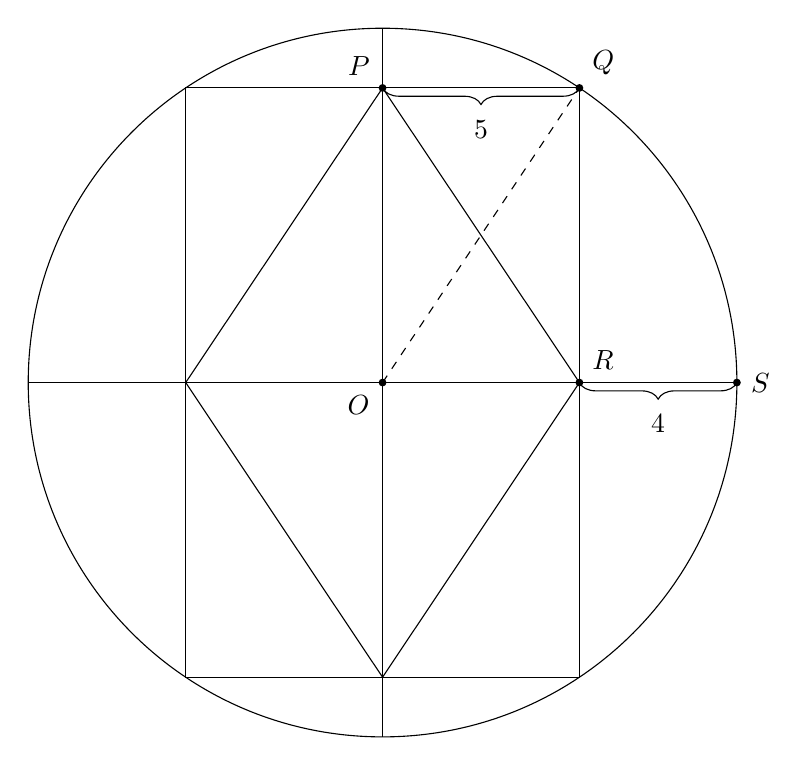
\begin{tikzpicture}[scale=0.5,dot/.style={circle,fill,inner sep=1pt}]
    \tikzmath{\y = 2 * sqrt(14);}
    \draw circle (9);
    \draw (9, 0) -- (-9, 0);
    \draw (0, 9) -- (0, -9);
    \draw[dashed] (0,0) -- (5, \y);
    \draw (5,\y) -- (-5, \y) -- (-5, -\y) -- (5, -\y) -- cycle;
    \draw (0, \y) -- (5, 0) -- (0, -\y) -- (-5, 0) -- cycle;

    % tikz code generated with help from gemini
    % Labels for the origin and the upper right sub-rectangle
    \node[dot, label={below left:$O$}] at (0,0) {};
    \node[dot, label={above left:$P$}] at (0, \y) {};
    \node[dot, label={above right:$Q$}] at (5, \y) {};
    \node[dot, label={above right:$R$}] at (5, 0) {};
    \node[dot, label={right:$S$}] at (9, 0) {};
    
    % Braces and Numerical Labels
    % Brace for the value 5 (Inside the top edge)
    \draw [decorate, decoration={brace, mirror, amplitude=6pt}] (0, \y) -- (5, \y) 
        node [midway, yshift=-15pt] {5};
        
    % Brace for the value 4 (On the horizontal diameter)
    \draw [decorate, decoration={brace, mirror, amplitude=6pt}] (5, 0) -- (9, 0) 
        node [midway, yshift=-15pt] {4};
\end{tikzpicture}

We know that point $O$ is the center of the circle that all lines that look perpendicular are perpendicular. 

By the fact that everything is perpendicular, we know that $PQRO$ is a rectangle. With this, $\overline{PQ}\cong \overline{OR}$, so $\text{length}(\overline{OR})=5$, and $\text{length}(\overline{OS})=\text{length}(\overline{OR}) + \text{length}(\overline{RS})=9$. Thus, the circle has radius $9$ since $\overline{OS}$ is a radius.

We can also show that $\Delta PQR \cong \Delta ORQ$ since $\overline{PQ} \cong \overline{OR}$, $\angle PQR \cong \angle ORQ$, and $\overline{QR}\cong \overline{RQ}$. By congruent triangles, we know that $\overline{PR} \cong \overline{OQ}$ and thus $\text{length}(\overline{PR})=\text{length}(\overline{OQ})$, but since $\overline{OQ}$ is a radius, we know that $\text{length}(\overline{OQ})=9$.

Thus, $\overline{PR}$, a side of the diamond, has length $9$.
\end{Solution} 

\vspace{1cm}

\begin{Solution}
{\bf (\S1.5, Problem 3)}\\
\begin{enumerate}[label=\alph*.]
    \item Because $P \implies Q \equiv Q\lor \lnot P$, we can use replacement to rewrite $P \implies Q \implies R$ as $\boxed{R \lor (\lnot Q) \lor (\lnot P)}$.
    \item By DeMorgan's laws, $P \lor Q \equiv \boxed{\lnot ((\lnot P) \land \lnot Q)}$.
    \item From part (b) and the replacement principle, we know that any expression involving $\lor$ can be written only using $\lnot$ and $\land$, as desired. To rewrite expressions involving $\implies$, we can apply $P \implies Q \equiv Q \lor \lnot P$ and then rewrite the $\lor$ using DeMorgan's laws (part b) to derive $P \implies Q \equiv \lnot(P \land \lnot Q)$. Thus, we have shown that $\lnot$ and $\land$ alone are an adequate set of logical connectives for expressing any expression involving $\lor$, $\land$, $\lnot$, or $\implies$.
\end{enumerate}
\end{Solution} 

\vspace{1cm}

\begin{Solution}
{\bf (\S1.5, Problem 4)}\\
First, a truth table for the Sheffer stroke/NAND:
\begin{tabular}{|c|c||c|}
\hline
$P$ & $Q$ & $P \uparrow Q$ \\ \hline
\false&\false&\true\\ \hline
\false&\true&\true\\ \hline
\true&\true&\false\\ \hline
\true&\false&\true\\ \hline
\end{tabular}

\begin{enumerate}[label=\alph*.]
    \item $\lnot P \equiv P \uparrow P$ \\ \begin{tabular}{|c||c|c|}
        \hline
        $P$ & $\lnot P$ & $P \uparrow P$ \\ \hline
        \false&\true&\true\\ \hline
        \true&\false&\false\\ \hline
        \end{tabular}
    \item $P \lor Q \equiv (P \uparrow P) \uparrow(Q \uparrow Q)$ \\ \begin{tabular}{|c|c||c|c|c|c|}
        \hline
        $P$ & $Q$ & $P \lor Q$ & $Q \uparrow Q$ & $P \uparrow P$ & $(P \uparrow P) \uparrow (Q \uparrow Q)$ \\ \hline
        \false&\false&\false&\true&\true&\false\\ \hline
        \false&\true&\true&\false&\true&\true\\ \hline
        \true&\true&\true&\false&\false&\true\\ \hline
        \true&\false&\true&\true&\false&\true\\ \hline
        \end{tabular}
    \item $P \land Q \equiv (P \uparrow Q) \uparrow(P\uparrow Q)$ \\ \begin{tabular}{|c|c||c|c|c|}
        \hline
        $P$ & $Q$ & $P \land Q$ & $P \uparrow Q$ & $(P \uparrow Q) \uparrow(P \uparrow Q)$ \\ \hline
        \false&\false&\false&\true&\false\\ \hline
        \false&\true&\false&\true&\false\\ \hline
        \true&\true&\true&\false&\true\\ \hline
        \true&\false&\false&\true&\false\\ \hline
        \end{tabular}
    \item $P \implies Q \equiv \boxed{P \uparrow(Q \uparrow Q)}$\\ 
        \begin{tabular}{|c|c||c|c|c|}
        \hline
        $P$ & $Q$ & $P \implies Q$ & $Q \uparrow Q$ & $P \uparrow (Q \uparrow Q)$ \\ \hline
        \false&\false&\true&\true&\true\\ \hline
        \false&\true&\true&\false&\true\\ \hline
        \true&\true&\true&\false&\true\\ \hline
        \true&\false&\false&\true&\false\\ \hline
        \end{tabular}
\end{enumerate}
\end{Solution} 

\vspace{1cm}

\begin{Solution}
{\bf (\S1.5, Problem 6)}\\
Given two sentential forms $S_1$ and $S_2$, the expression $S_1 \iff S_2$ is itself a new sentential form that evaluates to true whenever $S_1$ and $S_2$ both evaluate to the same value. However, the expression $S_1 \equiv S_2$ is a judgment of logical equivalence that is not itself a sentential form (it has no value), and it expresses the idea that for all possible values that the sentential variables within $S_1$ and $S_2$ can take on, $S_1 \iff S_2$ will evaluate to true (i.e. $S_1 \equiv S_2$ expresses that $S_1 \iff S_2$ is a tautology).
\end{Solution} 

\vspace{1cm}

\begin{Solution}
{\bf (\S1.5, Problem 8)}\\
\begin{enumerate}[label=\alph*.]
\item For all sentential forms $S_1$ and $S_2$, logical implication $S_1 \models S_2$ is a judgment that the corresponding material implication $S_1 \implies S_2$ is a tautology ($S_1 \implies S_2$ evaluates to true for all choices of sentential variables within $S_1$ and $S_2$). Again, while $S_1 \implies S_2$ is another sentential form that can be evaluated, $S_1 \models S_2$ has no value.
\item Logical implication $S_1 \models S_2$ and logical equivalence $S_1 \equiv S_2$ are both judgements that the underlying material versions are tautologies. While the judgment $S_1 \models S_2$ asserts that the sentential form $S_1 \implies S_2$ is a tautology, the judgment $S_1 \equiv S_2$ asserts that the sentential form $S_1 \iff S_2$ is a tautology.
\end{enumerate}
\end{Solution} 




\newpage{}
\section{Appendix}
Python code for generating truth tables:
(sorry I have been told that I do not code like a real person)
\begin{verbatim}
def graycode(n):
    arr = [False]*n
    ret = [arr[:]]
    for i in range(2**n-1):
        bits = (i+1)&~i
        bits &= ~(bits - 1)
        # print(bits.bit_length()-1)
        arr[n - 1 - (bits.bit_length() - 1)] ^= True
        ret.append(arr[:])
    return ret

def impl(a, b):
    return (not a) or b

def nand(a, b):
    return not (a and b)

bstr = lambda x: '\\true' if x else '\\false'

def latextt(novars, func):
    gc = graycode(novars)
    trial = func(*([False]*novars))
    print(f"\\begin{{tabular}}{{|{'c|'*novars}|{'c|'*len(trial)}}}")
    print("\\hline")
    print(f"$P_{'$ & $P_'.join(map(str, range(novars)))}$" +
          f" & $X_{'$ & $X_'.join(map(str,range(len(trial))))}$ \\\\ \\hline")
    for row in gc:
        res = func(*row)
        print('&'.join(map(bstr, row + res)) + '\\\\ \\hline')
    print("\\end{tabular}\n\n")

latextt(3, lambda p,q,r: [p and q, p or r, impl(p and q, p or r)])
latextt(2, lambda p,q: [impl(p, q), impl(p,q)==q, impl(impl(p,q)==q,p)])
latextt(2, lambda p,q: [impl(q, p), impl(q, impl(q, p)), impl(p, impl(q, impl(q, p)))])

print('nand')
latextt(2, lambda p,q: [nand(p, q)])
print('not')
latextt(1, lambda p: [not p, nand(p, p)])
print('or')
latextt(2, lambda p,q: [p or q, nand(q, q), nand(p, p), nand(not p, not q)])
print('and')
latextt(2, lambda p,q: [p and q, nand(p, q), not nand(p, q)])
print('impl')
latextt(2, lambda p,q: [impl(p, q), not q, nand(p, not q)])
\end{verbatim}




\newpage{}
And now for something completely random

% https://q.uiver.app/#q=WzAsMTIsWzAsMiwiXFx0ZXh0e01vcn1fXFxtYXRoY2Fse0J9KEYoQSksRihBKSkiXSxbMCwxLCJnOkYoQSlcXHRvIEIsZ1xcaW5cXG1hdGhjYWx7Qn0iXSxbMCw1LCJcXHRleHR7TW9yfV9cXG1hdGhjYWx7QX0oQSxHRihBKSkiXSxbMyw1LCJcXHRleHR7TW9yfV9cXG1hdGhjYWx7QX0oQSxHKEIpKSJdLFszLDIsIlxcdGV4dHtNb3J9X1xcbWF0aGNhbHtCfShGKEEpLEIpIl0sWzEsMywiXFx0ZXh0e2lkfV97RihBKX0iXSxbMiwzLCJnIl0sWzEsNCwiXFxldGFfQSJdLFsyLDQsIkdnXFxjaXJjXFxldGFfQT1cXHRhdV97QUJ9KGcpIl0sWzMsMSwiXFxldGE6MV9cXG1hdGhjYWx7QX1cXHRvIEdGIl0sWzAsMCwiRzpcXG1hdGhjYWx7Qn1cXHRvXFxtYXRoY2Fse0F9Il0sWzMsMCwiRjpcXG1hdGhjYWx7QX1cXHRvXFxtYXRoY2Fse0J9Il0sWzAsNCwiXFxtYXRoZnJha3tofV97RihBKX1nIl0sWzAsMiwiXFx0YXVfe0EsRihBKX0iLDJdLFs0LDMsIlxcdGF1X3tBQn0iXSxbMiwzLCJcXG1hdGhmcmFre2h9X0EgRyBnIiwyXSxbNiw4LCIiLDIseyJzdHlsZSI6eyJ0YWlsIjp7Im5hbWUiOiJtYXBzIHRvIn19fV0sWzUsNiwiIiwyLHsic3R5bGUiOnsidGFpbCI6eyJuYW1lIjoibWFwcyB0byJ9fX1dLFs1LDcsIiIsMCx7InN0eWxlIjp7InRhaWwiOnsibmFtZSI6Im1hcHMgdG8ifX19XSxbNyw4LCIiLDAseyJzdHlsZSI6eyJ0YWlsIjp7Im5hbWUiOiJtYXBzIHRvIn19fV1d
\begin{tikzcd}
	{G:\mathcal{B}\to\mathcal{A}} &&& {F:\mathcal{A}\to\mathcal{B}} \\
	{g:F(A)\to B,g\in\mathcal{B}} &&& {\eta:1_\mathcal{A}\to GF} \\
	{\text{Mor}_\mathcal{B}(F(A),F(A))} &&& {\text{Mor}_\mathcal{B}(F(A),B)} \\
	& {\text{id}_{F(A)}} & g \\
	& {\eta_A} & {Gg\circ\eta_A=\tau_{AB}(g)} \\
	{\text{Mor}_\mathcal{A}(A,GF(A))} &&& {\text{Mor}_\mathcal{A}(A,G(B))}
	\arrow["{\mathfrak{h}_{F(A)}g}", from=3-1, to=3-4]
	\arrow["{\tau_{A,F(A)}}"', from=3-1, to=6-1]
	\arrow["{\tau_{AB}}", from=3-4, to=6-4]
	\arrow[maps to, from=4-2, to=4-3]
	\arrow[maps to, from=4-2, to=5-2]
	\arrow[maps to, from=4-3, to=5-3]
	\arrow[maps to, from=5-2, to=5-3]
	\arrow["{\mathfrak{h}_A G g}"', from=6-1, to=6-4]
\end{tikzcd}
\[ \text{Hom}(F(A),B) \cong \text{Hom}(A,G(B))\]


\vspace{1in}
\begin{lstlisting}[language=lean]
-- contravariant hom functor!
theorem contrapos (a b : Prop): (a → b) → ¬b → ¬a :=
    fun f w => w ∘ f

theorem demorgan (a b : Prop): ¬(a ∨ b) ↔ ¬a ∧ ¬b :=
    Iff.intro (fun n => ⟨fun va => n <| Or.inl va, fun vb => n <| Or.inr vb⟩)
    (fun ⟨na, nb⟩ aob => aob.casesOn (fun va => na va) (fun vb => nb vb))

theorem otherdemorgan (a b: Prop): ¬a ∨ ¬b → ¬(a ∧ b) :=
    fun naob => naob.casesOn (fun na ⟨va, _⟩ => na va) (fun nb ⟨_, vb⟩ => nb vb)
\end{lstlisting}


\[ \mathrm{Hom}\left(\lim_{\longrightarrow} F,X\right) \cong \lim_{\longleftarrow}\left[\mathrm{Hom}(-,X)\circ F\right]\]
\[ \therefore \lnot (A\lor B) \cong ((\lnot A) \land \lnot B)\]
\end{document}
